%% Requires compilation with XeLaTeX or LuaLaTeX
\documentclass[aspectratio=169,10pt,xcolor={table,dvipsnames},t]{beamer}
\usetheme{UCBerkeley}
\hypersetup{colorlinks=true, linkcolor=blue, citecolor=blue, urlcolor=blue}
\usepackage{xcolor}

\title[lecture 02]{Next Generation Data Centers and Energy Management Systems}
\subtitle{Lecture 2B: Psychrometrics and Heat Transfer}
\author{Prof. Thomas M. Schutzius}
\institute{Department of Mechanical Engineering}
\date{Fall 2026}

\begin{document}

\begin{frame}
  \titlepage
\end{frame}

% Uncomment these lines for an automatically generated outline.
%\begin{frame}{Outline}
%  \tableofcontents
%\end{frame}

{
\setbeamertemplate{background}{} % Hides background for this frame
\setbeamertemplate{footline}{}   % Reclaims the bottom space
\smallframetitle
	\begin{frame}
		\frametitle{Learning Plan}
%		% Commands to include a figure:
		\begin{itemize}
			\item Introduction to Data Center Systems and Thermodynamics 
			\item \textbf{Psychrometrics and Heat Transfer}
			\item Performance Metrics and Standards 
			\item Applied Computational Fluid Dynamics (CFD)
			\item Liquid Cooling \& Advanced Heat Transfer 
			\item Chip Cooling: Heat Conduction and Thermal Interface Materials 
			\item Power Delivery and Infrastructure (Energy sources: Geothermal, Solar, Nuclear, etc.)
			\item Overview of Simulation Field; the Concept of a Digital Twin 
			\item Machine Learning and Optimization Tools 
			\item Modeling and Simulation of an Energy Management System 
			\item Control Systems and Optimization 
			\item Spacecraft Thermal Control
			\item Final Project Work, Peer Feedback, and Mentor Check-in 
			\item Symposium 
		\end{itemize}		
	\end{frame}
}

{
\setbeamertemplate{background}{} % Hides background for this frame
\setbeamertemplate{footline}{}   % Reclaims the bottom space
\smallframetitle
	\begin{frame}
		\frametitle{Learning Objectives}
%		% Commands to include a figure:
		\begin{itemize}
			\item Analyze a data center CRAC and rack using thermodynamic and psychrometric principles.
			\item Analyze the cooling system within the data center hall using a thermofluid flow network.
%			\item Define the ensemble coefficient of performance for a data center
		\end{itemize}		
	\end{frame}
}

{
\setbeamertemplate{background}{} % Hides background for this frame
\setbeamertemplate{footline}{}   % Reclaims the bottom space
\smallframetitle
\begin{frame}{Water-side economizer}
  \begin{columns}
    \begin{column}{0.48\textwidth}
		\begin{figure}
			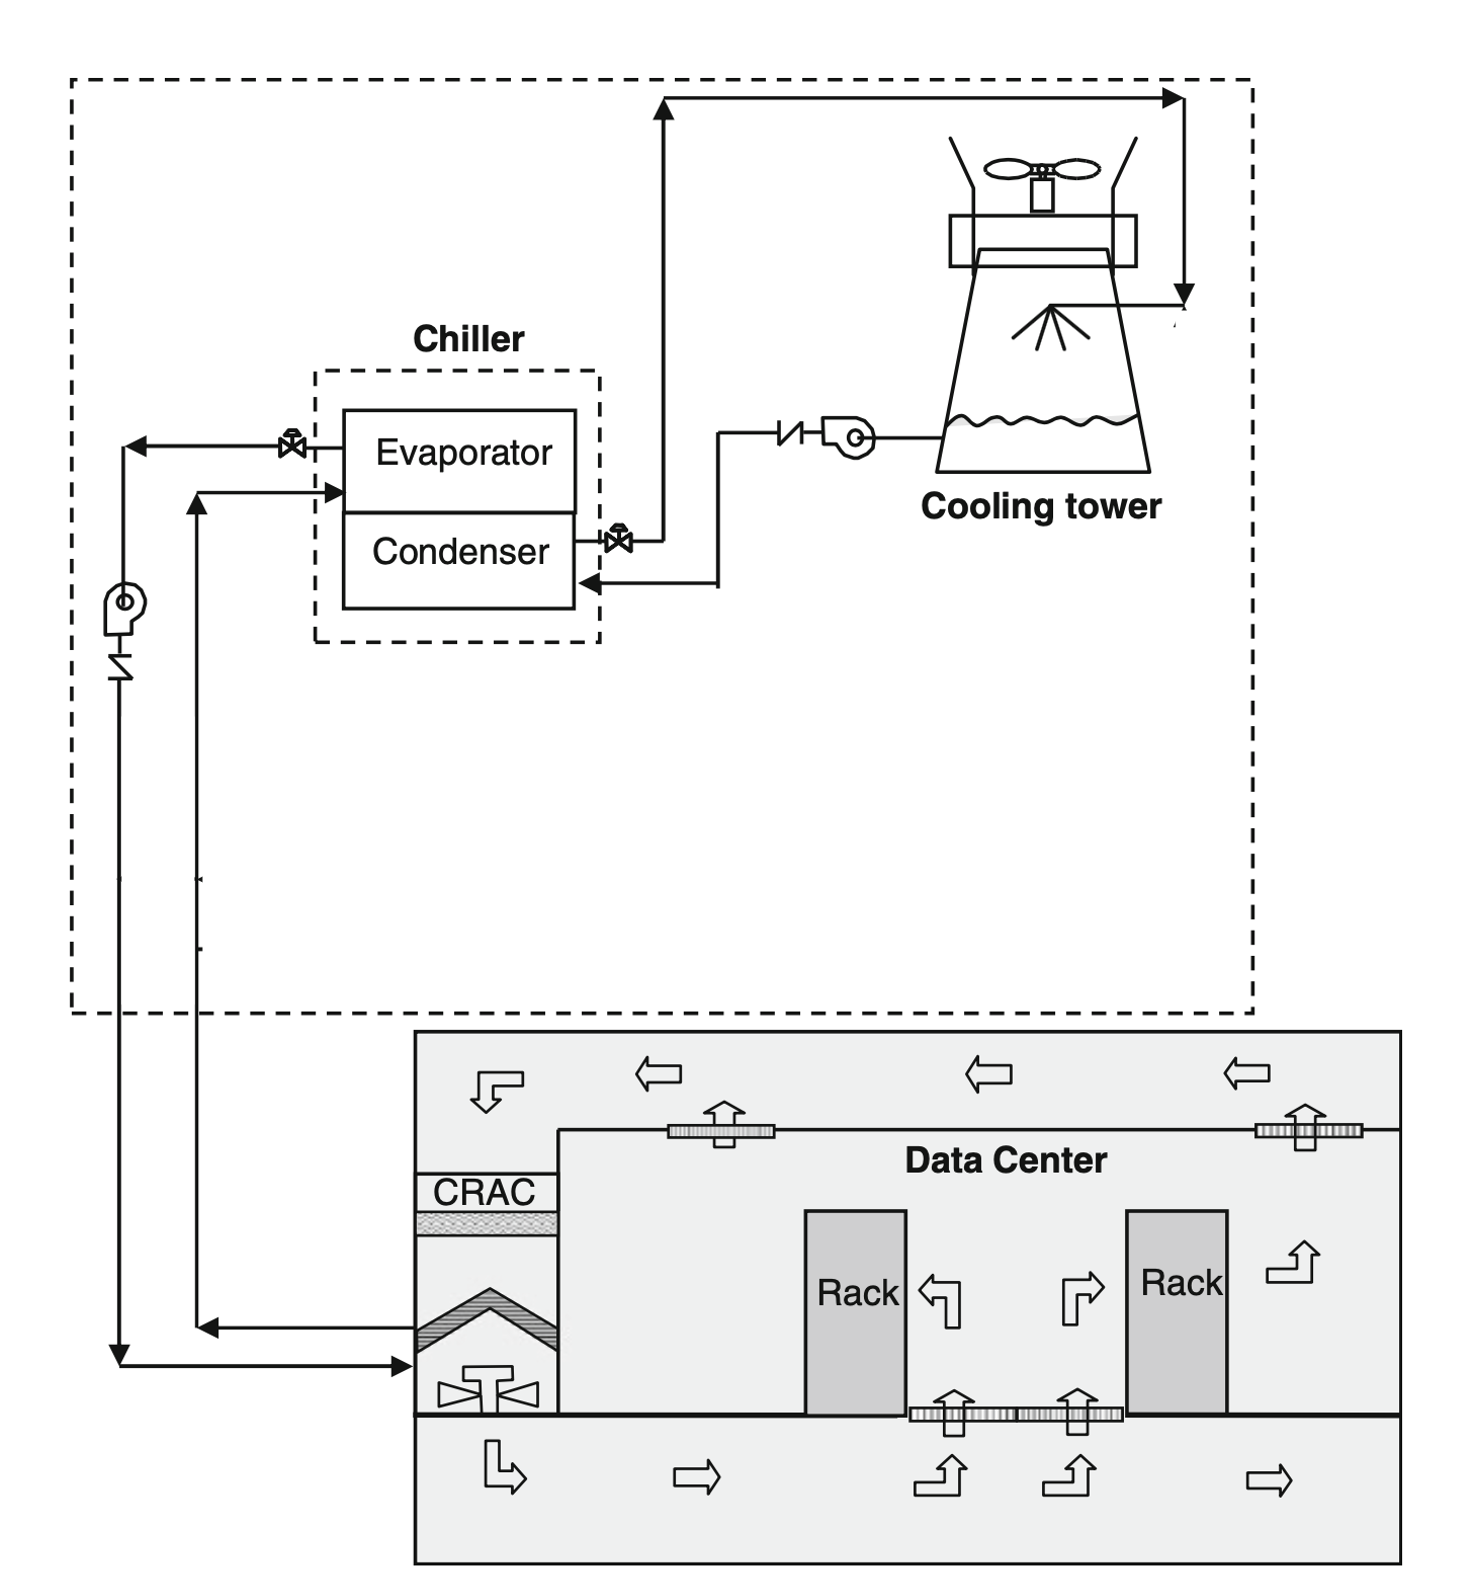
\includegraphics[width=0.7\textwidth]{../figures/joshi2021energy-figure-02-53-removed.png}
%			\vspace{-0.5cm}
		 \caption{No economizer (Figure 2.53 in Ref. \cite{joshi2012energy}).}
		\end{figure}
    \end{column}

    \begin{column}{0.48\textwidth}
		\begin{figure}
			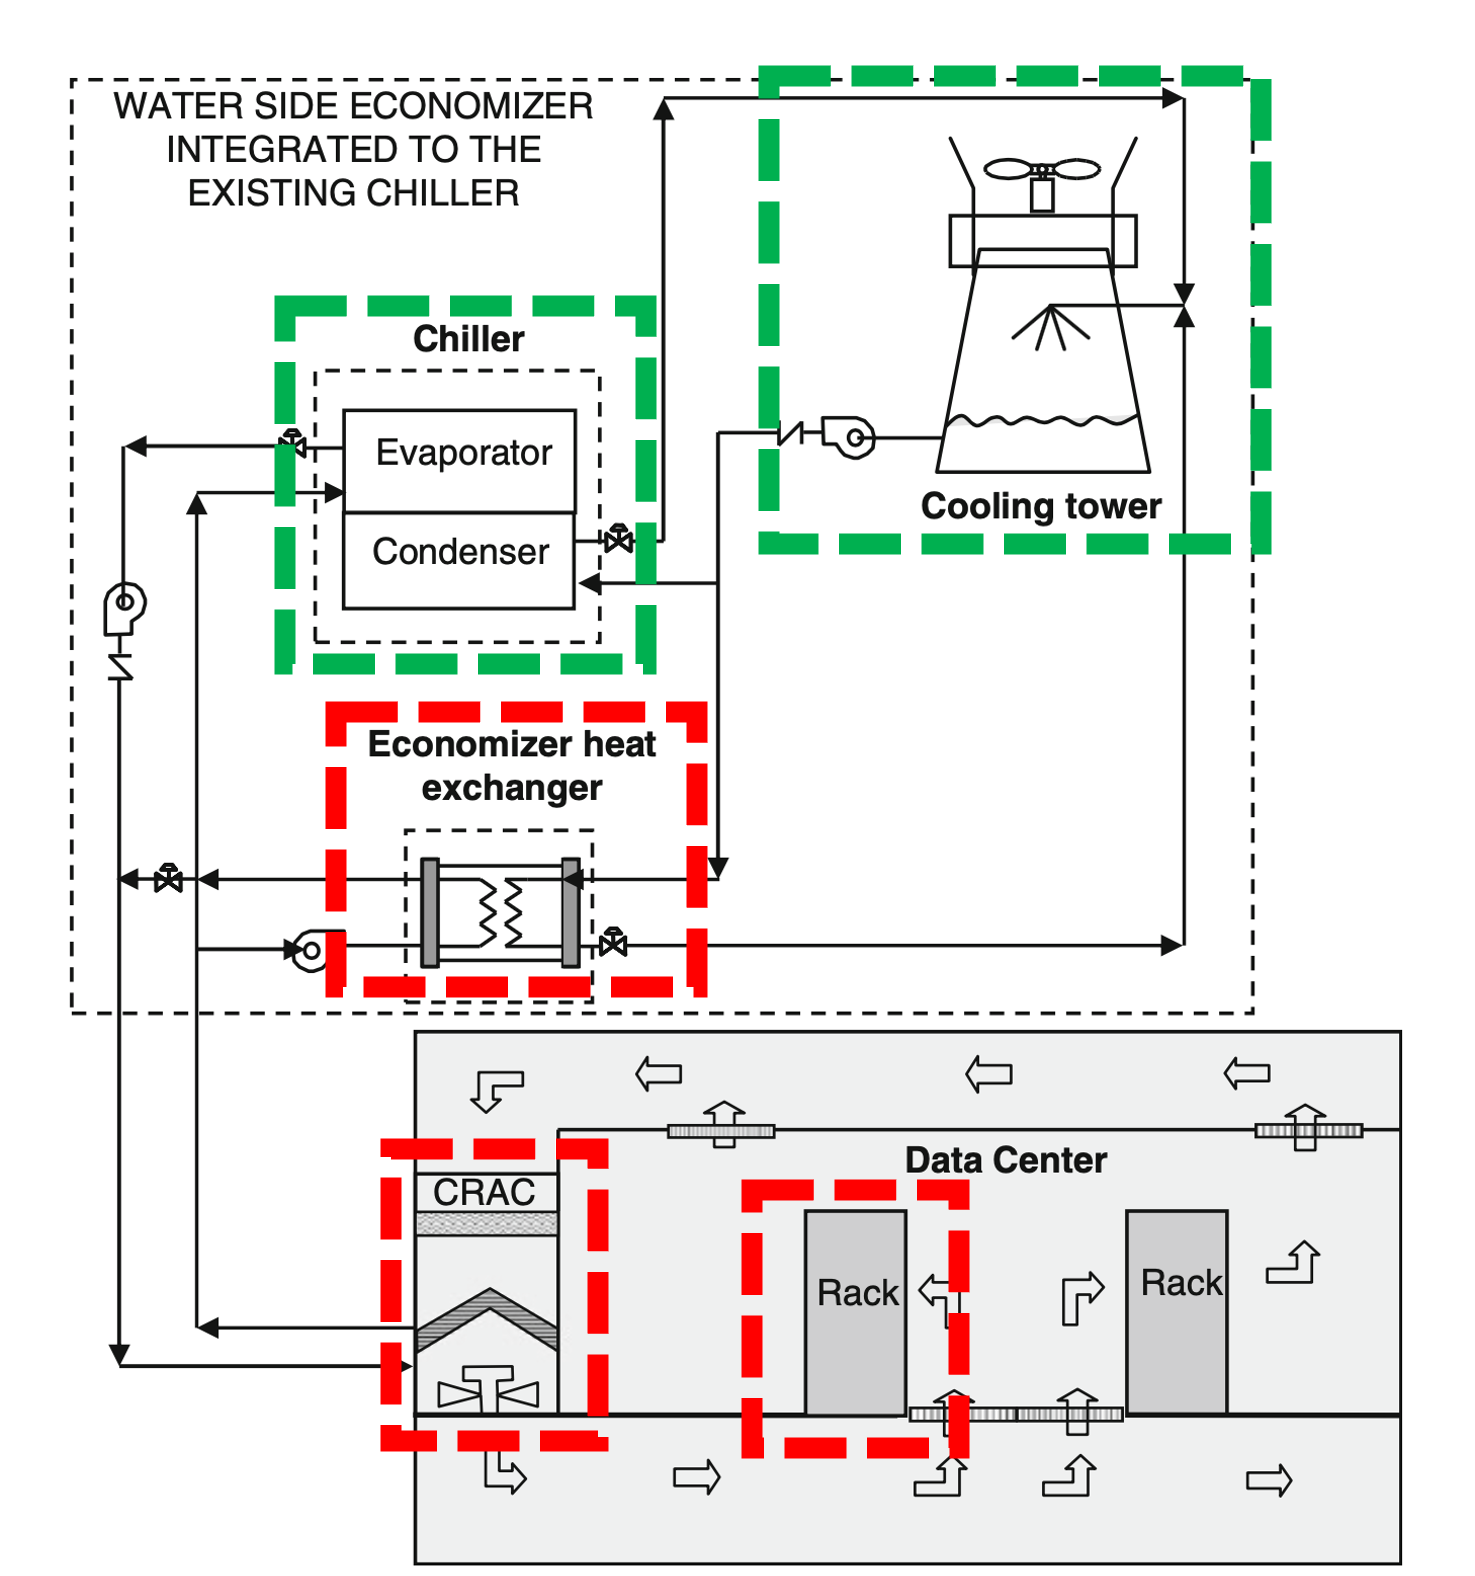
\includegraphics[width=0.7\textwidth]{../figures/joshi2021energy-figure-02-53-highlighted.png}
%			\vspace{-0.5cm}
		 \caption{Water-economizer (Figure 2.53 in Ref. \cite{joshi2012energy}).}
		\end{figure}
    \end{column}
  \end{columns}
\end{frame}
}

{
\setbeamertemplate{background}{} % Hides background for this frame
\setbeamertemplate{footline}{}   % Reclaims the bottom space
\smallframetitle
	\begin{frame}
		\frametitle{\href{https://datahub.berkeley.edu/user-redirect/git-pull?repo=https://github.com/mtsn-lab/me137-237a&subPath=examples/crac.ipynb}{Energy analysis of a CRAC}}
%			\begin{itemize}
%				\item Standard 90.1-2025 -- Energy Standard for Data Centers: \href{https://ashrae.iwrapper.com/ASHRAE_PREVIEW_ONLY_STANDARDS/STD_90.4_2025}{Link}. You need to register in order to read. You can also become a student member of ASHRAE. There is a Golden Gate chapter. 
%		\end{itemize}
	\end{frame}
}

{
\setbeamertemplate{background}{} % Hides background for this frame
\setbeamertemplate{footline}{}   % Reclaims the bottom space
\smallframetitle
	\begin{frame}
		\frametitle{\href{https://datahub.berkeley.edu/user-redirect/git-pull?repo=https://github.com/mtsn-lab/me137-237a&subPath=examples/simpleHeating.ipynb}{Energy analysis of a rack}}
%			\begin{itemize}
%				\item Standard 90.1-2025 -- Energy Standard for Data Centers: \href{https://ashrae.iwrapper.com/ASHRAE_PREVIEW_ONLY_STANDARDS/STD_90.4_2025}{Link}. You need to register in order to read. You can also become a student member of ASHRAE. There is a Golden Gate chapter. 
%		\end{itemize}
	\end{frame}
}

{
\setbeamertemplate{background}{} % Hides background for this frame
\setbeamertemplate{footline}{}   % Reclaims the bottom space
\smallframetitle
	\begin{frame}
		\frametitle{\href{https://datahub.berkeley.edu/user-redirect/git-pull?repo=https://github.com/mtsn-lab/me137-237a&subPath=examples/flowNetworkTheory.ipynb}{Flow network theory}}
%			\begin{itemize}
%				\item Standard 90.1-2025 -- Energy Standard for Data Centers: \href{https://ashrae.iwrapper.com/ASHRAE_PREVIEW_ONLY_STANDARDS/STD_90.4_2025}{Link}. You need to register in order to read. You can also become a student member of ASHRAE. There is a Golden Gate chapter. 
%		\end{itemize}
	\end{frame}
}

{
\setbeamertemplate{background}{} % Hides background for this frame
\setbeamertemplate{footline}{}   % Reclaims the bottom space
\smallframetitle
	\begin{frame}
		\frametitle{\href{https://datahub.berkeley.edu/user-redirect/git-pull?repo=https://github.com/mtsn-lab/me137-237a&subPath=examples/flowNetworkCoolingDataHall.ipynb}{Flow network analysis of a data center hall}}
%			\begin{itemize}
%				\item Standard 90.1-2025 -- Energy Standard for Data Centers: \href{https://ashrae.iwrapper.com/ASHRAE_PREVIEW_ONLY_STANDARDS/STD_90.4_2025}{Link}. You need to register in order to read. You can also become a student member of ASHRAE. There is a Golden Gate chapter. 
%		\end{itemize}
	\end{frame}
}

%{
%\setbeamertemplate{background}{} % Hides background for this frame
%\setbeamertemplate{footline}{}   % Reclaims the bottom space
%\smallframetitle
%	\begin{frame}
%		\frametitle{Energy analysis of heat transfer from a cabinet}
%			\begin{itemize}
%				\item In addition to maintaining the inlet air temperatures, data centers also need to adhere to the humidity levels specified by ASHRAE guidelines.
%				\item ASHRAE: American Society of Heating, Refrigerating and Air-Conditioning Engineers
%				\item The relevant technical committee is: TC 9.9 (Mission Critical Facilities, Data Centers, Technology Spaces and Electronic Equipment): The flagship committee for data centers. TC 9.9 sets global industry standards for thermal guidelines. 
%				\item Standard 90.1-2025 -- Energy Standard for Data Centers: \href{https://ashrae.iwrapper.com/ASHRAE_PREVIEW_ONLY_STANDARDS/STD_90.4_2025}{Link}. You need to register in order to read. You can also become a student member of ASHRAE. There is a Golden Gate chapter. 
%		\end{itemize}
%	\end{frame}
%}

%{
%\setbeamertemplate{background}{} % Hides background for this frame
%\setbeamertemplate{footline}{}   % Reclaims the bottom space
%\smallframetitle
%\begin{frame}{The ideal vapor-compression refrigeration cycle}
%  \begin{columns}
%    \begin{column}{0.48\textwidth}
%		\begin{figure}
%			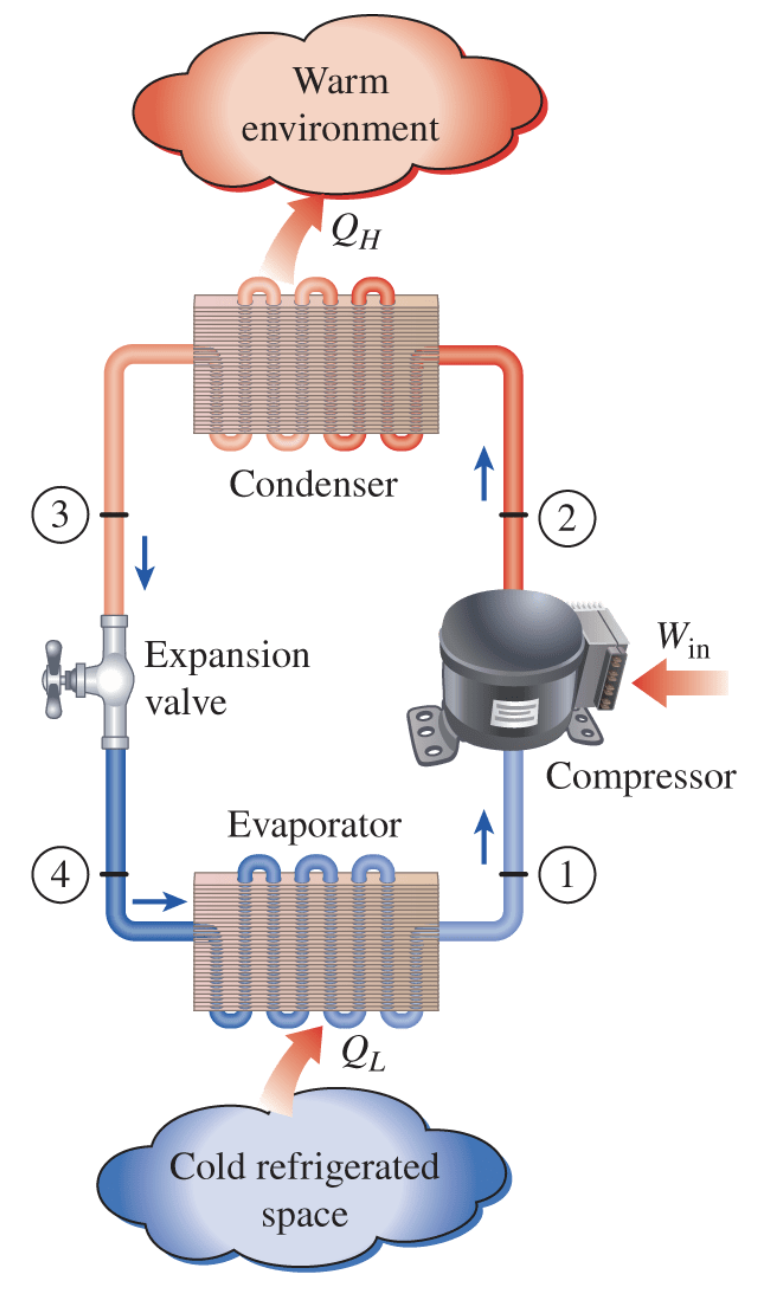
\includegraphics[width=0.5\textwidth]{../figures/cengel2019thermodynamics-figure-11-3.png}
%%			\vspace{-0.5cm}
%		 \caption{\label{fig:refrigeration-system}Reproduced from Figure 11.3 in Ref. \cite{cengel2019thermodynamics}.}
%		\end{figure}
%    \end{column}
%
%    \begin{column}{0.48\textwidth}
%		\begin{figure}
%			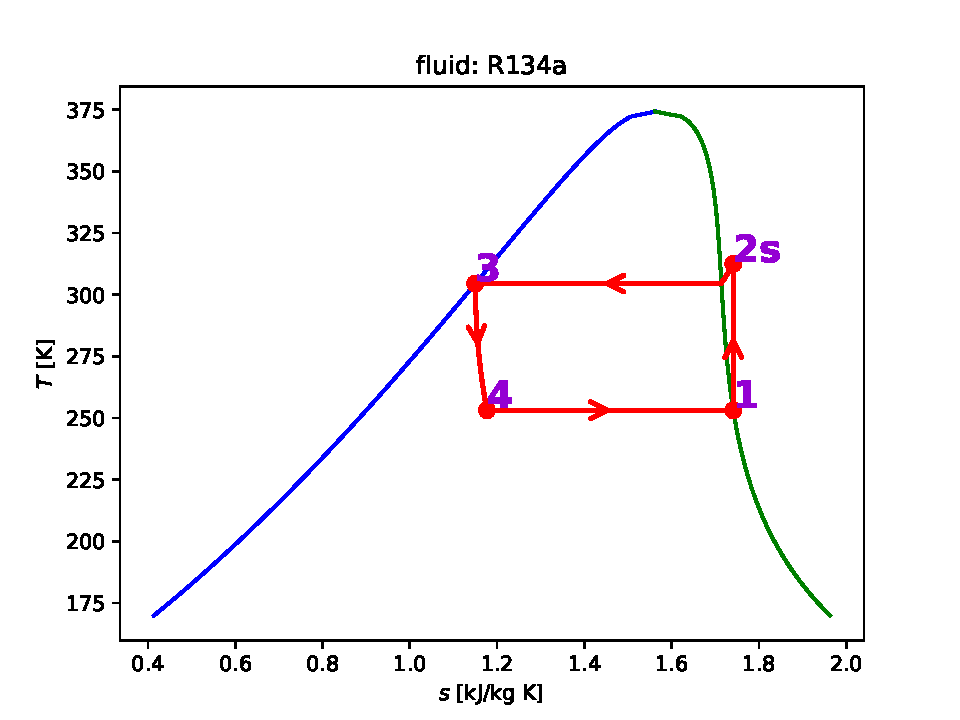
\includegraphics[width=1\textwidth]{../figures/refrigerationCycleR134a_Ts.pdf}
%%			\vspace{-0.5cm}
%		 \caption{\label{fig:refrigeration-system}Generated from \href{https://datahub.berkeley.edu/user-redirect/git-pull?repo=https://github.com/mtsn-lab/me40&subPath=scripts/refrigerationCycleR134a.ipynb}{here}.}
%		\end{figure}
%    \end{column}
%  \end{columns}
%\end{frame}
%}



{
\setbeamertemplate{background}{} % Hides background for this frame
\setbeamertemplate{footline}{}   % Reclaims the bottom space
\setbeamertemplate{bibliography item}[text] % Replaces default icons with numbers
\smallframetitle
	\begin{frame}[allowframebreaks]{References}
		\bibliographystyle{plain}
		\bibliography{../../bibliography}
	\end{frame}
}

%{
%\setbeamertemplate{background}{} % Hides background for this frame
%\setbeamertemplate{footline}{}   % Reclaims the bottom space
%\smallframetitle
%\begin{frame}
%\frametitle{Teaching team}
%
%\begin{columns}[T]
%
%\begin{column}{0.48\textwidth}
%\small
%Ben Brown
%
%		\begin{figure}
%			
\includegraphics[width=0.5\textwidth]{figures/ben-brown.pdf}
%			\vspace{-0.5cm}
%%		\caption{\label{fig:ben-brown}\href{https://eta-publications.lbl.gov/sites/default/files/2024-12/lbnl-2024-united-states-data-center-energy-usage-report.pdf}{eta-publications.lbl.gov}}
%		\end{figure}
%
%
%\end{column}
%
%\begin{column}{0.48\textwidth}
%Amelia Stacey
%
%		\begin{figure}
%			
\includegraphics[width=0.5\textwidth]{figures/oski.jpeg}
%			\vspace{-0.5cm}
%%		\caption{\label{fig:ben-brown}\href{https://eta-publications.lbl.gov/sites/default/files/2024-12/lbnl-2024-united-states-data-center-energy-usage-report.pdf}{eta-publications.lbl.gov}}
%		\end{figure}
%\end{column}
%
%\end{columns}
%\end{frame}
%}




\end{document}
